\documentclass[12pt]{report}
\usepackage[utf8]{inputenc}
\usepackage[T1]{fontenc}
\usepackage[french]{babel}
\usepackage[toc,page]{appendix} 
\usepackage{graphicx}
\usepackage{geometry}
\usepackage{xcolor}
\usepackage{tikz}
\usetikzlibrary{positioning}
\definecolor{processblue}{cmyk}{0.96,0,0,0}

\usepackage{lipsum}
\usepackage{titlesec}
\usepackage{sectsty}
\usepackage{eurosym}
\usepackage{listings}
\usepackage[backend=bibtex,sorting=none]{biblatex}
\addbibresource{bibliography.bib}

\renewcommand{\baselinestretch}{1.05}
\usepackage{fancyhdr}
\pagestyle{fancy}
\fancyhead[LO]{\bfseries\nouppercase{\rightmark}}
\setlength{\headheight}{15pt}

\fancypagestyle{plain}{
  \fancyhead{}
  \fancyfoot[C]{\thepage}
  \renewcommand{\headrulewidth}{0pt}
}

\geometry{top=2.5cm, bottom=3.5cm, left=3cm , right=2cm}
\renewcommand{\thechapter}{\Roman{chapter}}
\renewcommand{\thesection}{\Alph{section}}

\newcommand{\LMUTitle}[9]{
  \thispagestyle{empty}
  \vspace*{\stretch{1}}
  {\parindent0cm
   \rule{\linewidth}{.7ex}}
  \begin{flushright}

    \vspace*{\stretch{1}}
    \sffamily\bfseries\Huge
    #1\\
    \vspace*{\stretch{1}}
    \sffamily\bfseries\large
    #2
    \vspace*{\stretch{1}}
  \end{flushright}
  \rule{\linewidth}{.7ex}
  \vspace*{\stretch{5}}
  \begin{center}
    
\includegraphics[width=3in]{UPN-logo.jpg}
  \end{center}
  \vspace*{\stretch{1}}
  \begin{center}\sffamily\LARGE{#3}\end{center}
  \newpage
  \thispagestyle{empty}
}

\begin{document}

  \LMUTitle
      {Les faux profils\\
      sur les réseaux sociaux\\
      et leurs moyens de détection}              
      {Lucas Nayet}                       
      {Mémoire Master 2 MIAGE - Juin 2019}                          
\thispagestyle{empty}

\setcounter{page}{}
\chapter*{Remerciements}
J'adresse mes remerciements à toute la formation du Master MIAGE classique pour l'enseignement qu'elle m'a apporté. J'adresse plus particulièrement mes remerciements pour Monsieur Pascal Poizat, responsable du master MIAGE classique et pour Monsieur Jean-François Pradat-Peyre, mon tuteur de Master 2, pour l'aide et le temps qu'ils m'ont consacré. 

\makeatletter
\def\@makechapterhead#1{%
  \vspace*{50\p@}%
  {\parindent \z@ \raggedright \normalfont
    \Huge \bfseries #1\par\nobreak
    \vskip 40\p@
  }}
\makeatother

\renewcommand{\contentsname}{Sommaire}
{\tableofcontents}

\chapter{Introduction}
Les relations humaines se sont vues être profondément transformées ces trente dernières années avec l'apparition d'Internet en 1990 qui s'est imposé en 10 ans comme étant le réseau de télécommunication incontournable. Avec lui, s'est vu apparaître nombre de nouveaux services et notamment le réseau social, qui est aujourd'hui devenu un moyen de communication incontournable, principalement chez les jeunes, bien que ce phénomène concerne aussi les personnes plus âgés.\\

Le réseau social a radicalement changé notre manière de communiquer, il est désormais possible de communiquer avec des individus vivant à l'autre bout du pays et même à l'autre bout du monde, de connaître, apprécier, aimer des personnes que l'on aurait jamais pu connaître auparavant et de nouer ce que l'on appelle des relations "virtuelles" avec ces individus parfois plus fortes que des relations réelles. \\


Les réseaux sociaux font source de débats divers, principalement autour de la vie privée de l'utilisateur, de la santé psychologique de ce dernier, ou encore de la frontière entre vie réelle et vie privée de plus en plus floue que ces dits réseaux font. \\

Par ailleurs, diverses controverses sont apparues avec les réseaux sociaux mettant en péril la vie privée et la sécurité des utilisateurs notamment les faux comptes et les faux profils. Ce mémoire trouve sa raison d'être autour de ces deux dimensions, mais avant d'aller plus loin, on va d'abord s'intéresser au contexte et aux concepts généraux du sujet.\\

\chapter{Contexte et concepts}
\section{Les médias sociaux}
Les réseaux sociaux appartiennent à une grande catégorie que l'on appelle les médias sociaux. Les médias sociaux sont des applications web qui permettent la création et la publication de contenus générés par l’utilisateur et le développement de réseaux sociaux en ligne en connectant les profils des utilisateurs. Le secteur d'activité des médias sociaux sont les médias, internet, le marketing et la communication numérique.\\

Le terme recouvre les différentes activités qui intègrent la technologie, l’interaction sociale, et la création de contenu. Les médias sociaux utilisent l’intelligence collective dans un esprit de collaboration en ligne. Par le biais de ces moyens de communication sociale, des individus ou des groupes d’individus forment un réseau social4, collaborent, créent ensemble du contenu Web, organisent le contenu, l’indexent, le modifient ou font des commentaires, le combinent avec des créations personnelles. \\

Les termes Web 2.0 et médias sociaux demeurent assez proches et concernent une grande variété de sites différents : les blogs, les wikis, et les réseaux sociaux numériques de tout type. Les médias sociaux utilisent beaucoup de techniques, telles que les flux RSS et autres flux de syndication Web. \\

Pour l'historique, le développement des médias sociaux remonte à la fin des années 1970. Deux passionnés d’informatique conçoivent le Computerized Bulletin Board System en 1978. Il s’agit du premier site permettant aux internautes d’échanger des informations (notes, réunions…) par voie informatique. Par la suite, des étudiants de l’Illinois développent Mosaic, le premier navigateur web permettant d’afficher le World Wide Web. \\

En page suivante, se trouve une figure représentant les différents types de médias sociaux, on peut ainsi constater qu'ils sont très diversifiés. 

\begin{figure}
\begin{center}
    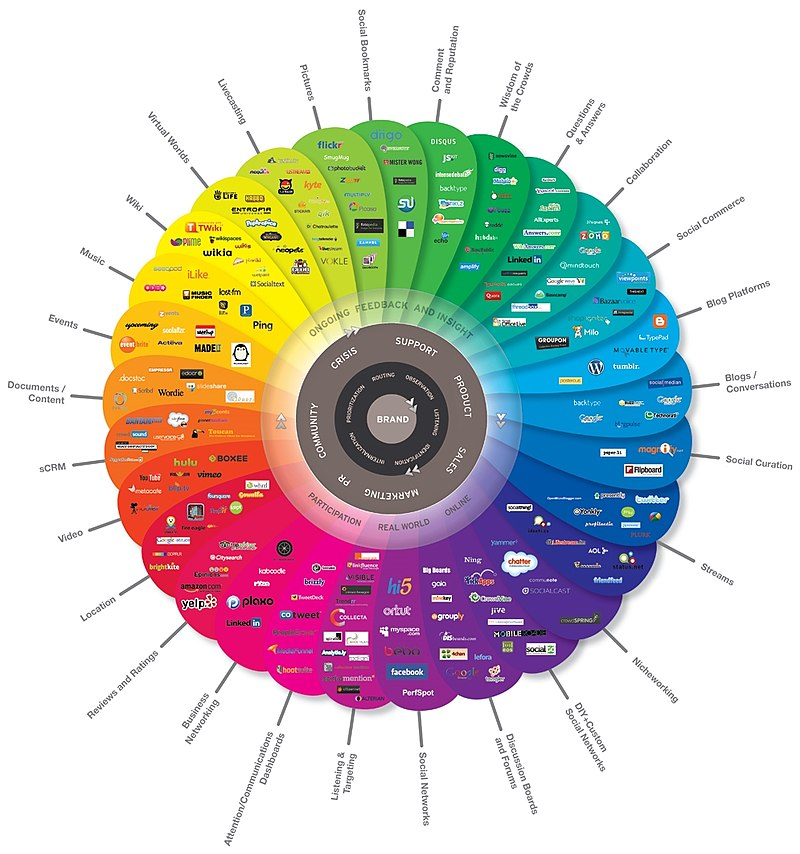
\includegraphics[width=180mm]{MediasSociaux.jpg}
    \end{center}
    \caption{Les différents types de médias sociaux}
\label{fig:les différents types de médias sociaux}
  \end{figure}

\newpage 
\section{Les réseaux sociaux}
Ainsi, au vu de ce qui a été dit précédemment et au vu de la figure de la page précédente, les réseaux sociaux ne sont qu’une sous-partie des médias sociaux. En sciences humaines et sociales, l'expression réseau social désigne \textit {"un agencement de liens entre des individus et/ou des organisations, constituant un groupement qui a un sens : la famille, les collègues, un groupe d'amis, une communauté..."} \\
L'expression a été introduite en 1954 par l'anthropologue australien John Arundel Barnes. Andreas Kaplan et Michael Haenlein définissent le réseau social comme \textit{"un groupe d’applications en ligne qui se fondent sur la philosophie et la technologie du net et permettent la création et l’échange du contenu généré par les utilisateurs".}\\

Deux grands phénomènes se dégagent de la notion de réseau social en terme de science social : la règle des 150 et le phénomène du petit monde. \\
Selon Wikipédia, en ce qui concerne la règle des 150, la psychologie évolutionniste forme l'hypothèse qu'il existe un nombre maximal de personnes qu'un individu puisse reconnaître et dont il puisse interpréter les réactions. 
Selon l'anthropologue britannique Robin Dunbar, un être humain peut entretenir une relation humaine stable avec au plus 148 personnes, un nombre généralement arrondi à 150. Au-delà de ce nombre, limité par les capacités et l'organisation cérébrales, des institutions structurées par des règles doivent intervenir.\\
Toujours selon Wikipédia, la « règle de 150 », aussi appelée « nombre de Dunbar » limite la taille d'un réseau social. Si le groupe est plus nombreux, la relation de confiance s'en trouve affectée. \\
Quant au phénomène du petit monde, il s'agit de l'hypothèse que la longueur de la chaîne des connaissances sociales requise pour lier une personne arbitrairement choisie à n'importe quelle autre sur Terre est généralement courte. Le concept a engendré l'expression célèbre des "six degrés de séparation" après l'expérience du petit monde de 1967, réalisée par le psychologue Stanley Milgram. Il conclut qu'en moyenne, il n'y a que six intermédiaires entre deux êtres humains sur la terre.\\

Hors du domaine des sciences sociales, l'expression réseau social renvoie aux entreprises de réseautage social sur internet et à leurs utilisateurs à travers le monde. Les applications désignées comme "service de réseautage social en ligne" servent à constituer un réseau social virtuel en reliant, non pas des personnes, mais des identités virtuelles. Leurs utilisateurs utilisent des liens hypertexte ou des bases de données dont ils n'ont parfois pas connaissance dans le but de faciliter la gestion des carrières professionnelles, la distribution et la visibilité artistique ou les rencontres privées. Certains réseaux sociaux sont devenues de véritables entreprises de communication qui peuvent cibler un public très large. \\

Pour l'histoire, bien que le premier réseau social ayant fait décoller la popularité de ce phénomène soit Facebook, apparu en 2004 pour des étudiants américains et généralisé à tous en 2006, le tout premier réseau social est bien apparu en 1995 et il s'agit de Classmates, et il existe encore aujourd'hui. L’objectif de ce site était de remettre en contact des anciens camarades de classe. Ce réseau social a réussi à compter 50 millions d'utilisateurs, mais l'arrivée de Facebook aura eu raison de son existence médiatique, si bien qu'aujourd'hui, peu de personnes connaissent l'existence de ce réseau social, qui est pourtant l'ancêtre du réseau social tel qu'on le connaît aujourd'hui. 

\begin{figure}[h]
    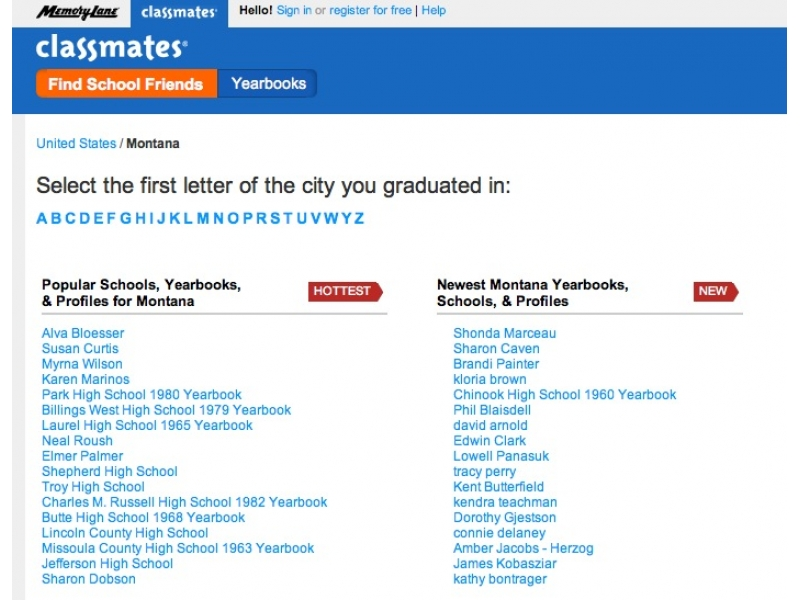
\includegraphics[width=180mm]{navigation-dans-classmates.jpg}
    \caption{Page d'accueil de Classmates}
\label{fig:Page d'accueil de Classmates}
  \end{figure}

\section{Enjeux et problématique}
Les réseaux sociaux subissent de plein fouet le phénomène de faux comptes et de faux profils.  Pour information, Facebook recense 270 millions de faux comptes et profils en 2018, et Twitter aurait 48 millions de comptes et profils fake.\\

Ce phénomène est un véritable fléau. Un commerce d'achat et de ventes de faux profils sévit sur Twitter, dans le but de vendre de la publicité via le large nombre d’abonnés. \\

Il est urgent d'agir pour les réseaux sociaux et de lutter contre ce phénomène tant l'ampleur et la dangerosité potentielle que ce dernier prend sont importantes.\\ 

Ainsi, les enjeux de ce mémoire vont se faire autour des profils et des comptes fakes que l'on va irrémédiablement trouver sur les réseaux sociaux et également leurs moyens de détection existants à ce jour. \\ 

Pour répondre à ces enjeux, l'identité numérique d'une personne va être très importante. En effet, avec la multitude de réseaux sociaux existant à ce jour et l'importance que cela peut prendre dans la vie d'une personne, l'identité numérique et les conséquences qui en découlent vont être décisives, et sont directement liées aux faux comptes et aux faux profils.\\

On s'intéressera d'abord à la notion de faux comptes et de faux profils et la différence entre les deux. Puis, on s'attardera sur les faux profils malveillants et les méthodes existantes à ce jour pour les débusquer. Enfin, j'apporterai mon apport au niveau des méthodes pour déceler un faux profil ainsi qu'une critique sur le sujet.

\chapter{Faux comptes et profils}
La frontière entre les faux comptes et les faux profils peut paraître floue au premier abord, non à tort. Des similitudes existent entre ces deux types de fakes, mais il existe également des différences qui vont être décisives. 

\section{Les faux comptes}
Un faux compte est un compte automatisé. Il appartient à la catégorie de ce que l'on appelle les bots ou robots. Ce genre de comptes est extrêmement populaire et on en trouve sur tous les réseaux sociaux. Dans le cadre de ce mémoire, nous allons prendre deux types de bots qui répondent à eux deux aux différentes finalités d'un bot : les bots Twitter et les bots Discord. \\

\subsection{Premier exemple : les bots Twitter}
Un bot ou robot Twitter est un compte Twitter automatisé. Un bot Twitter peut répondre à différents objectifs selon sa nature. \\

Un bot Twitter peut être d’abord utilisé pour des stratégies d’influence ou de manipulation de type astroturfing. Selon la définition Wikipedia, l'astroturfing désigne des techniques de propagande manuelles ou algorithmiques utilisées à des fins publicitaires ou politiques ou encore dans les campagnes de relations publiques, qui ont pour but de donner une fausse impression d'un comportement spontané ou d'une opinion populaire sur Internet. Il s’agit alors de faux comptes Twitter qui vont automatiquement diffuser des contenus plus ou moins véridiques destinés à influencer l’audience du réseau social. Selon une étude de l’université de Londres « City », près de 13 500 faux comptes Twitter auraient ainsi influencé la sortie lors du référendum du Brexit en 2017.\\

Un robot Twitter peut également être utilisé pour animer automatiquement un compte en retweetant par exemple tous les tweets comprenant un mot clé ou une expression. Dans ce cas, le compte peut être réel, mais une grande partie de son fonctionnement est automatisé avec éventuellement un système de validation des publications. L’usage vise alors à se positionner comme expert en donnant l’illusion d’avoir une activité de veille soutenue. \\

Dans d’autres cas, des bots Twitter peuvent être utilisés pour bâtir artificiellement des audiences de followers par des pratiques de mass following automatisés ou pour pratiquer de la veille. \\

Pour terminer cette section sur les bots Twitter, il me semblait pertinent de s'attarder sur l'un d'entre eux, que je trouve à la fois sympathique et intéressant. Le compte @PkmnCheckerBot corrige un utilisateur (dans les heures qui viennent généralement) qui fera une faute sur l'orthographe français d'un Pokémon. En voici la preuve : 

\begin{figure}[h]
    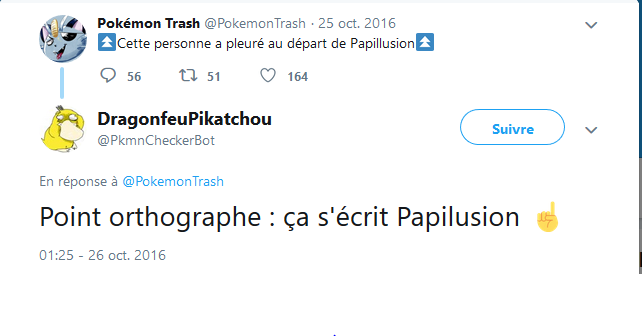
\includegraphics[width=180mm]{BotTwitterPokemon2.PNG}
    \caption{Exemple de correction orthographique du bot Pokémon}
\label{fig:Exemple de correction orthographique du bot Pokémon}
  \end{figure}
  
Ainsi, on voit bien le procédé employé par ce bot. Ici, Pokémon Trash, qui pour information, est l'un des sites Pokémon les plus connus, si ce n'est le plus connu, se fait corriger l'orthographe du Pokémon Papilusion, qui ne prend qu'un seul "l". Ce bot fait, tous les mois, le bilan de nombre de Pokémon qu'il a eu besoin de corriger ainsi que le nombre de fois qu'il a dû en corriger un, comme on peut le constater à la page suivante :

\begin{figure}[h]
    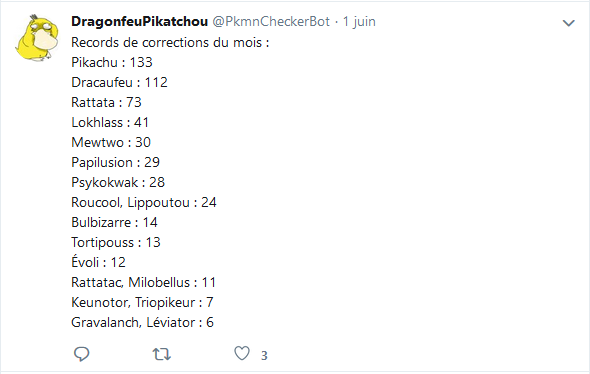
\includegraphics[width=180mm]{BotTwitterPokemon3.PNG}
    \caption{Bilan mensuel du bot Pokémon}
\label{fig:Bilan mensuel du bot Pokémon}
  \end{figure}
  
\newpage
Dernier point très important que je souhaite vous montrer au sujet de ce bot : sa biographie Twitter. Présente en page suivante, on apprend ainsi qu'il s'agit d'un robot mais surtout qu'il a été codé par un humain. Pour une question de droit, j'ai préféré masquer la personne ayant codé ce bot. Cette caractéristique de codage est présente dans tout bot et est essentielle pour le qualifier de tel. On comprend aussi que le bot n'a aucune volonté de cacher son identité de robot puisqu'il affiche son statut de bot clairement dans sa bio. Bien que cela ne soit pas toujours le cas, un bot est en général facilement identifiable par un utilisateur.

\begin{figure}[h]
    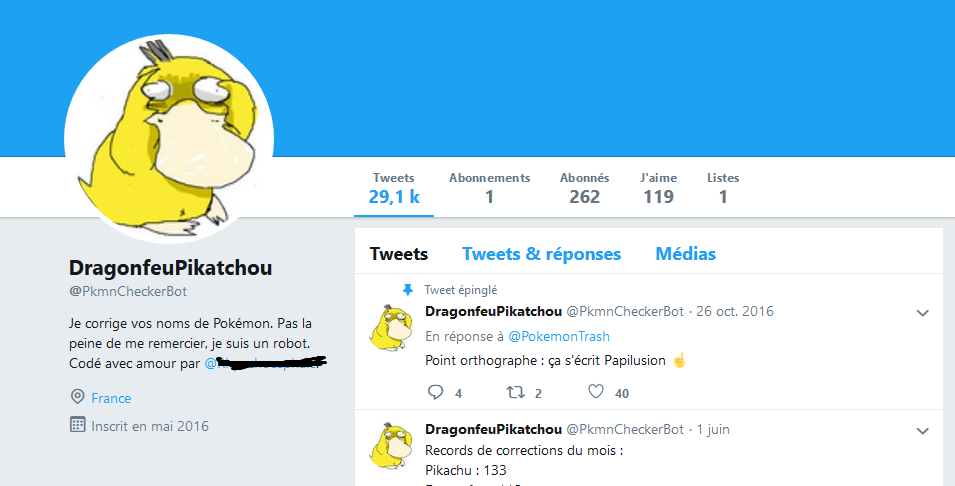
\includegraphics[width=220mm]{BotTwitterPokemon.PNG}
    \caption{Biographie du bot Pokémon}
\label{fig:Biographie du bot Pokémon}
  \end{figure}
  
\newpage
\subsection{Second exemple : les bots Discord}
Discord est un logiciel gratuit de VoIP conçu initialement pour les communautés de joueurs. Il fonctionne sur les systèmes d’exploitations Windows, macOS, Linux, Android, iOS ainsi que sur les navigateurs web. Le succès grandissant de ce réseau social l'élargi aujourd'hui à d'autres communautés comme les développeurs. \\ 

Le grand succès de Discord vient notamment du fait que l'on puisse créer son propre serveur, serveur comportant différents salons avec lesquels on peut discuter d'un sujet en particulier ce qui le rend meilleur pour grand nombre d'utilisateurs que ses concurrents directs comme Skype. Il est possible d'installer différents bots sur son serveur Discord qui permettent différentes utilités, ces bots possèdent bien un identifiant à quatre chiffres comme toute personne inscrite sur Discord doit posséder pour avoir un compte, les bots Discord sont donc bien des comptes. Le bot MEE6 (qui est le plus célèbre et populaire du logiciel) permet de rendre d'abord le serveur plus attractif, avec un système de montées de niveaux qui encourage l'activité. Ce même bot permet également d'afficher à partir d'une commande, un texte que l'administrateur du serveur aura au préalable écrit. Cela peut se révéler très utile par exemple dans le cadre d'un tournoi ou une compétition, où il suffirait de taper une commande "!regles" (toute commande de ce bot commence par un !) pour que le bot affiche toutes les règles du tournoi ou de la compétition. MEE6 peut également permettre de gérer le serveur en l'absence du propriétaire de ce dernier. \\

Il existe une multitude d'autres bots sur Discord : Pokécord permet de capturer des Pokémon sur son propre serveur, Septapus permet d'afficher les conversations du serveur sous forme de bande dessinées... \\

Ci-dessous, les logos des bots Discord MEE6 et Septapus. 

\begin{figure}[h]
    \begin{center}
    
\includegraphics[width=30mm]{Mee6Discord.png}
    \end{center}
    \begin{center}
    
\includegraphics[width=30mm]{SeptapusDiscord.png}
    \end{center}
    \caption{Logo des Bots Discord MEE6 et Septapus}
\label{fig:Logo des Bots Discord MEE6 et Septapus}
  \end{figure}

Ainsi, les faux comptes que l'on trouve sur les réseaux sociaux portent également le nom de bot ou robot. Ils sont programmées par une personne humaine et ont un but différent selon le réseau où ils sont. Les faux comptes sont facilement reconnaissables et n'ont pas pour but de tromper un utilisateur quant à la réalité de ce dernier, ils sont là pour proposer des services, faire de la publicité... \\
Cependant, ils peuvent tout de même avoir un but d'influence et de manipulation des utilisateurs, notamment politique, mais dans le cadre de ce mémoire, les moyens de détection des faux comptes ne vont pas être une priorité de part leur facilité à être débusqués, même à l'oeil nu, et leur non-malveillance d'autre part. Il n'en est pas de même pour les faux profils.

\section{Les faux profils}
Un faux profil contrairement à un faux compte, est "géré" par une personne humaine. C'est les informations qui sont saisies dans le profil qui posent problème pour établir la véracité de ce dernier.

\subsection{L'identité numérique d'un individu}
Pour définir la notion de faux profils, il faut reprendre la notion d'identité numérique. L'identité numérique, c'est l'ensemble des contenus publiés sur Internet qui permettent de définir un individu, et ce, que la personne soit physique ou morale. Cela regroupe ainsi les commentaires que l'on laisse, les opinions que l'on expose, les publications que l'on partage, les achats que l'on effectue, nos coordonnées, notre réseau (qui l'on a dans nos contacts), nos loisirs, notre réputation à savoir ce qui est dit sur nous... \\

Ces informations, laissées au fil des navigations, sont collectées par les moteurs de recherche, comme Google, et sont rendues public.
Cette identité sur Internet a donc une influence sur la e-réputation, sur la façon dont les internautes perçoivent une personne. En résumé, l’identité numérique est l’image que vous renvoyez sur Internet, votre image virtuelle, dématérialisée.
L'e-réputation, c'est donc l'image renvoyée par la perception de ces contenus. L'identité numérique regroupe aujourd'hui des contenus mis en ligne sur divers espaces, et notamment sur les médias sociaux : blogs personnels, profils sur les réseaux sociaux, contenus partagés, commentaires... On distingue généralement deux types de contenus : ceux maîtrisés par la personne concernée (publiés par elle) et ceux non-maîtrisés par la personne concernée (publiés par un tiers). \\

Cette identité virtuelle se crée par le biais des réseaux sociaux, comme Facebook ou Twitter, ou des publications sur un blog. Les sites web de tous les genres construisent également notre identité, grâce à laquelle vous pouvez donc être connu et avoir une présence en ligne. Mais ces données, qui se retrouvent à la portée de tous, constituent un risque permanent pour les utilisateurs et pour la protection de leur vie privée. \\

En page suivante, se trouve une image qui regroupe sous forme de figure les différentes caractéristiques de l'identité numérique et permet ainsi de bien résumer les propos précédents. 

\begin{figure}[h]
    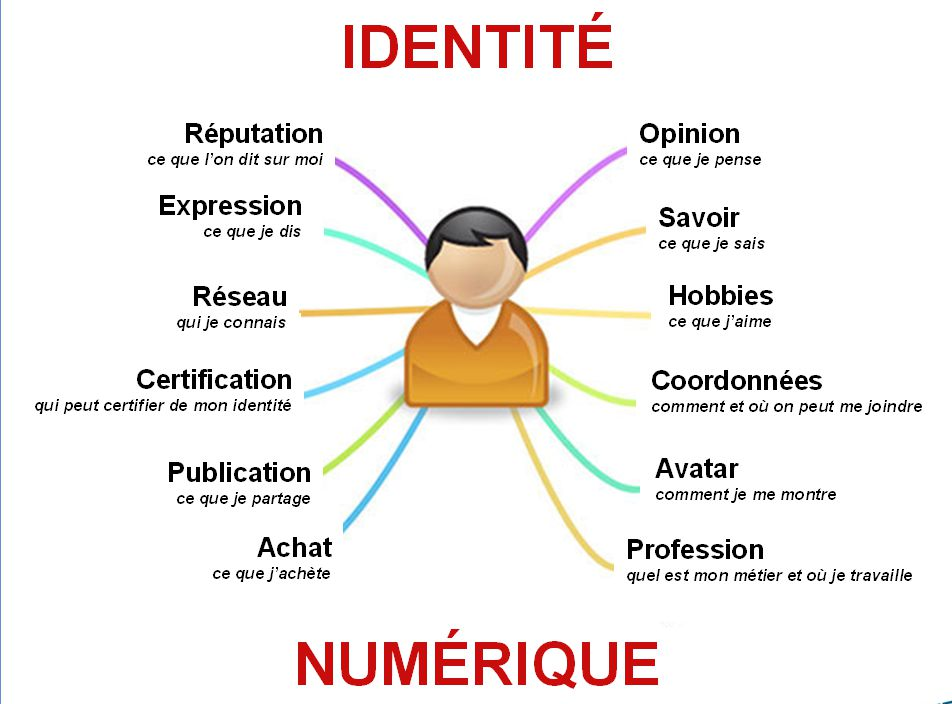
\includegraphics[width=180mm]{identite_num.png}
    \caption{Les différentes caractéristiques de l'identité numérique}
\label{fig:Les différentes caractéristiques de l'identité numérique}
  \end{figure}

\newpage
\subsection{Les risques et dérives de l'identité numérique}
\subsubsection{Les risques}
L'identité numérique comporte des risques allant de la simple exposition à des risques beaucoup plus complexes et graves.\\
Aujourd’hui, les informations inscrites sur Internet sont très difficiles à effacer. C’est pour cette raison qu’il est préférable de bien réfléchir avant de laisser une trace numérique afin d’éviter toutes les conséquences négatives d’une mauvaise e-réputation.\\

Il faut savoir que les traces laissées en ligne par soi-même et les traces laissées en ligne par d'autres internautes sont très importantes. On pense notamment à la recherche d'emploi. Selon l'enquête Questions Emploi réalisée par RegionsJob en 2014,  52\% des recruteurs font des recherches en ligne sur les candidats. Pour 31\% d'entre eux, l'e-réputation d'un candidat a déjà permis d'être recruté. Mais une mauvaise e-réputation peut également compromettre les chances d'un candidat : 35\% des recruteurs qui font ce type de recherches en ligne ont déjà écarté un candidat à cause de son identité numérique.\\

Ainsi, notre identité numérique a une conséquence directe sur l'image que l'on renvoie et cela, même en dehors du monde virtuel. En effet, l'apparence prime sur les réseaux sociaux et les gens sont de plus en plus victimes du fait de vouloir paraitre mieux que son voisin. Selon un récent sondage, 20\% des français choisissent leur lieu de vacances en fonction du fait qu'il soit "instagrammable" ou non. De plus, les commentaires que l'on laisse, les images que l'on poste, les informations personnelles que l'on affiche sur les réseaux sociaux ont une conséquence directe sur l'image que les autres perçoivent de nous, et cela a une conséquence non seulement sur Internet mais également dans la réalité, tant les réseaux sociaux rendent la frontière entre vie privée et vie publique floue. \\

L'un des derniers grands risques autour de l'identité numérique concerne le vol d'identité de ce dernier. Ce n’est pas un phénomène nouveau. Ce type d’escroquerie sur internet, visant à se faire passer pour un autre (entreprise, administration, personne physique) pour accéder à des données ou des comptes bancaires et détourner des fonds, ou porter atteinte à la réputation d’une entreprise ou d’une personne physique s’est développé parallèlement à l’essor de l’internet. \\

L’usurpation d’identité (numérique ou non) est constituée quand elle porte sur l’identité même de la victime (nom, prénom, surnom, pseudonyme, identifiants électroniques) ou sur toute autre donnée de nature à l’identifier. Cette dernière expression permet de s’affranchir de la notion de données à caractère personnel, au sens de la loi Informatique et Libertés, et de rechercher tous autres éléments permettant une identification. Il est donc possible d’y inclure les adresses IP, les URL, les mots de passe, ainsi que des logos, images, voire même un avatar, tous ces éléments permettant de pointer vers une personne physique. L’usurpation d’identité “numérique”, telle que prévue à l’article 226-4-1 al. 2 du code pénal, est commise sur un réseau de communication au public en ligne, ce qui comprend notamment les courriers électroniques, les sites web, les messages publiés en ligne et les profils en ligne sur les réseaux sociaux (Facebook, Twitter). L’usurpation d’identité numérique peut porter préjudice à deux catégories de victimes :

- la personne dont l’identité a été usurpée : l’auteur de l’infraction nuit à son image, à sa réputation, à sa marque ou trouble sa tranquillité. \\
- le tiers trompé : l’auteur de l’infraction induit l’internaute en erreur et lui soutire des informations et/ou de l’argent. \\

L’usurpation d’identité numérique est généralement commise de deux manières : par la technique du phishing (ou hameçonnage), ou par la création d’un faux site web ou d’un faux profil sur un service de réseau social. \\

Le phishing ou hameçonnage : le cyber-escroc usurpe l’identité d’un tiers, généralement une entreprise (banque, opérateur téléphonique) ou une administration, en communiquant via un faux courrier électronique et/ou via un site web contrefait. L’escroc reproduit alors les identifiants visuels et graphiques de la marque, en vue d’obtenir de la part d’internautes trompés, des informations personnelles (identifiants, mots de passe ou coordonnées bancaires). Ces informations sont ensuite utilisées pour accéder à leurs comptes et effectuer des opérations sous l’identité de l’internaute (virement, souscription d’un crédit, abonnement).\\

Dans le cas de la création d’un faux site web ou d’un faux profil sous l’identité d’une tierce personne, l’usurpation d’identité numérique est également réalisée via la création d’un faux site web, reprenant à l’identique les composants d’un site “légitime” (charte graphique, reproduction de tout ou partie du contenu, etc.). Cette technique est souvent liée à une “campagne” de phishing.\\

La création d’un faux site web ou d’un faux profil a pour objet ou pour effet de porter atteinte à l’honneur ou à la réputation du titulaire du site ou du profil, personne physique ou morale. \\

\begin{figure}[h]
    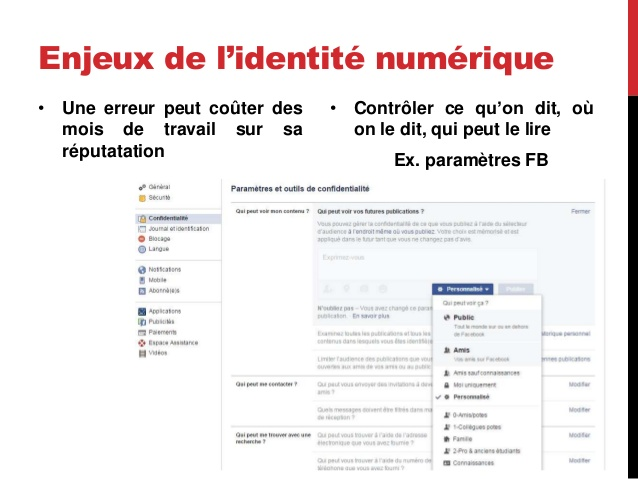
\includegraphics[width=150mm]{EnjeuxIdentiteNumerique.jpg}
    \caption{Les enjeux de l'identité numérique}
\label{fig:Les enjeux de l'identité numérique}
  \end{figure}

\newpage
\subsubsection{Les dérives}
Bien que l'identité numérique comporte des risques pour un individu qui ne maîtrise pas la sienne dans un monde où Internet est maître, l'usurpation d'identité étant le risque le plus courant et le plus préoccupant, certains utilisent la leur afin de se glorifier, de passer incognito, ou encore de se faire passer pour quelqu'un d'autre. Et pour cela, certains ont justement recours à l'usurpation d'identité en se faisant passer pour quelqu'un d'autre. Dans ce cas-là, la dérive découle du risque.\\

Nous avons vu précédemment que l'identité numérique d'une personne peut être utilisée lors du processus de recrutement par les recruteurs. Ainsi, un individu qui a conscience de cela, va avoir tendance à utiliser son identité numérique afin de se montrer sous son meilleur jour, tout en n'hésitant pas à masquer ou arranger certaines réalités voire mentir.\\

Cela peut encore aller plus loin avec des individus qui se créent une identité sur un réseau social dans le but d'escroquer des gens, via une arnaque à la webcam. Grâce à ces faux profils, ils rentrent en contact avec leurs futures victimes, usurpant l’identité d’un homme ou d’une femme dont ils ont récupéré les photos sur Internet. Le mode opératoire de l’arnaque à la webcam est alors classique, installer un climat de confiance sur une période plus ou moins longue,  dans le but d’obtenir à un moment des informations personnelles et des photos ou vidéos intimes. Derrière un chantage s'installe alors, la personne ayant piégé réclame alors de l'argent à la personne piégée sous peine de divulguer les photos ou vidéos intimes à sa famille ou ses amis.\\

Certains pédophiles attirent même leurs proies en créant un faux profil : ils se font passer pour une personne mineure dans le but de piéger leur interlocuteur, qui va alors penser qu'il parle à une personne de son âge afin d'obtenir des photos ou vidéos intimes, voire même d'organiser une rencontre afin de violer leur victime.

\begin{figure}[h]
\begin{center}
    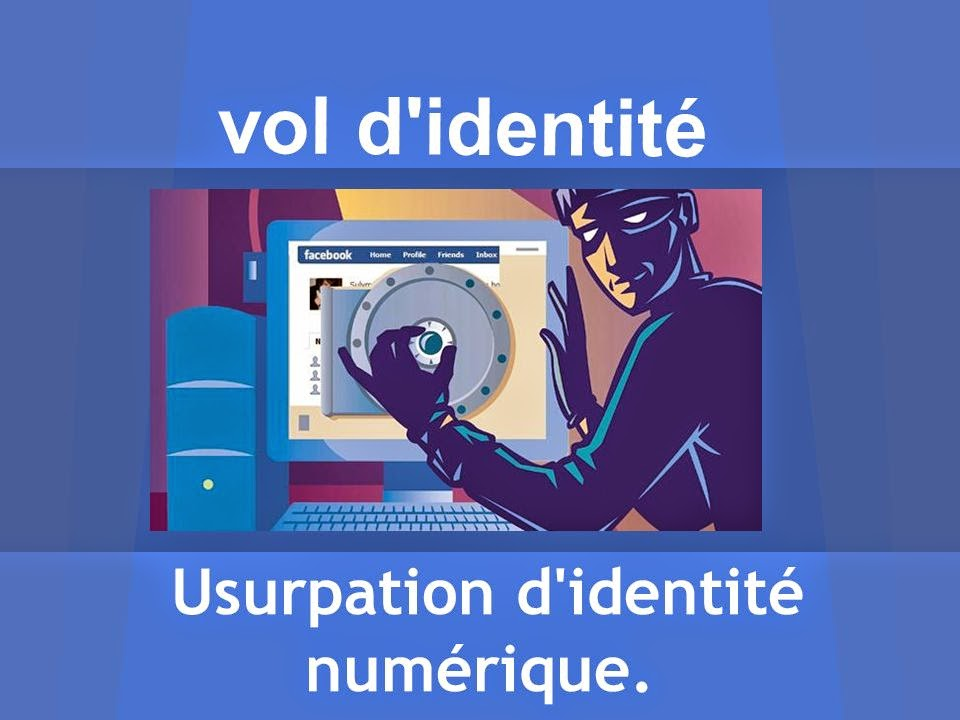
\includegraphics[width=150mm]{UsurpationIdentiteNumerique.jpg}
    \end{center}
    \caption{L'usurpation de l'identité numérique, un fléau}
\label{fig:L'usurpation de l'identité numérique, un fléau}
  \end{figure}

\newpage
\section{Notion de malveillance}
Ainsi, un faux profil est un profil dont les informations et/ou photos ne correspondent pas à ce que la personne est en réalité. \\

On peut distinguer trois types de faux profils : \\ 
- les personnes commanditées par des agences matrimoniales ou entreprises de speed dating.\\
- les personnes qui souhaitent conserver leur anonymat sur les sites de rencontres.\\
- les arnaqueurs, escroqueries sentimentales, arnaques à la webcam, pédophiles.\\

Si le deux premiers types de faux profils sont certes malhonnêtes, il n’y a pas vraiment de grand danger puisque dans le premier cas, les personnes commanditées sont généralement payées par une agence matrimoniale pour prospecter des clients. Les comptes associés à cet archétype s’apparentent donc à une forme de publicité qui permet à l’agence d’attirer les membres d’un site de rencontres. Quant au second type de profil, il concerne des personnes en couple qui désirent rester anonymes sur les sites de rencontres. Souvent sans danger, les personnes derrière ces profils veulent seulement rencontrer d’autres personnes en toute discrétion. En revanche, le troisième type de faux profil est bien plus préoccupant et est dans un but malveillant. Saboter des réputations, escroquer de l'argent, usurper des identités... ce phénomène se trouve surtout sur Facebook avec les harponneurs venant surtout d'Afrique de l'Ouest mais également avec les pédophiles, se faisant passer pour une personne jeune pour piéger leur victime.\\ 

Ainsi, contrairement aux faux comptes robots, les faux profils peuvent être dans un but malveillant que cela soit pour récupérer des fonds, arnaquer des particuliers ou même violer des victimes dans le cas des pédophiles. La notion de tromper son interlocuteur est également très importante pour établir la notion de faux profil malveillant : c'est notamment ce qui sépare un simple profil utilisé ayant un prénom et un nom faux dans le but de rester incognito d'un profil qui est utilisé par une personne qui cherchera à entrer en contact avec d'autres utilisateurs dans le but de tromper les autres utilisateurs. \\

Il est important ici de distinguer le caractère malhonnête du caractère malveillant, un fake malveillant sera malhonnête, la réciproque est en revanche fausse. En effet, certains bots Twitter sont malhonnêtes, cherchant à manipuler les foules pour des raisons politiques par exemple, mais ne sont pas pour autant malveillants, ils ne vont pas chercher à porter atteinte à une réputation ou encore à escroquer un tiers. \\

Quoi qu'il en soit, les réseaux sociaux cherchent à lutter contre ce phénomène qui prend une ampleur de plus en plus préoccupante, mais les moyens de lutte restent bien compliqués encore à ce jour.

\chapter{Méthodes de détection}

On a vu précédemment que les faux profils sont un phénomène qui n'échappent à aucun réseau.\\
Pour être clair dès le début, la méthode miracle pour déceler un faux profil n'existe pas. Les moyens de lutte restent extrêmement âpres. On peut les regrouper en deux catégories : la méthode naïve, qui est en réalité une méthode non-informatique et la méthode informatique, qui est bien entendu la plus intéressante dans le cadre du mémoire.\\

\section{La méthode naïve}
Il s'agit de méthodes qu'une personne un minimum observatrice sera en mesure de faire. Ces méthodes ne sont évidemment pas fiables à 100\% et dans le cas où la personne derrière le faux profil est une professionnelle, ce genre de méthodes risque d'échouer. Néanmoins, ce genre de méthodes permettent de déceler un faux profil facilement dans le cas où l'individu qui le contrôle est un amateur. Voici un regroupement des méthodes "naïves" les plus utilisées et les plus fiables pour mettre un faux profil à jour.  

\subsubsection{Recherche Google Images}
Une première méthode qui peut permettre de déceler un faux profil de manière très rapide, la recherche par Google Images. Il s’agit d’un outil incorporé dans Google, qui vous permet de comparer rapidement la photo de profil de la personne suspecte avec les propositions du moteur de recherche. Pour cela, glissez l’image du faux profil (enregistrée au préalable dans votre ordinateur) dans la barre de recherche Google Image, et vous verrez les images similaires détectées par Google ainsi que la liste des sites ayant publié cette image. Notons que cette technique n’est pas infaillible à 100\%, mais vous pouvez néanmoins essayer d’autres sites de comparaison d’images. Au passage, soulignons également que la plupart des faux profils (et faux comptes également) n’ont qu’une seule photo de profil. Aparté non négligeable, un faux compte peut aussi être débusqué de cette manière.
Ci-dessous, l'outil Google Images permettant d'effectuer cette manoeuvre.

\begin{figure}[h]
\begin{center}
    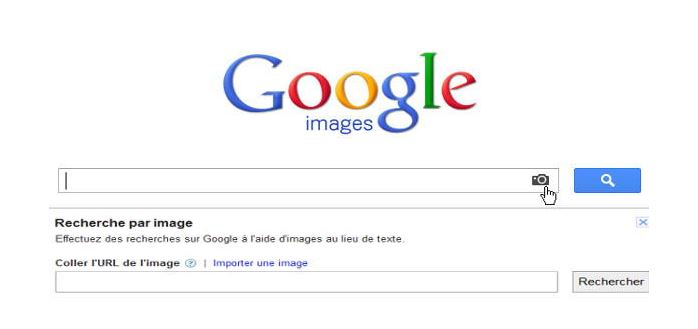
\includegraphics[width=150mm]{google-image-recherche.jpg}
    \end{center}
    \caption{Méthode Google Images de détection de faux profils}
\label{fig:Méthode Google Images de détection de faux profils}
  \end{figure}

\subsubsection{Obtenir l’adresse IP de votre interlocuteur}
Il est possible de piéger quelqu'un afin de connaître son adresse IP, sa localisation, ou d'autres informations. En localisant votre escroc, vous saurez par exemple s’il est en France ou dans un pays exotique. Un grand nombre d'escroqueries se base là-dessus car la personne ne vous dira pas la vérité sur sa localisation. Ainsi, vous serez en mesure d'établir la véracité du profil suspect avec cette méthode. Néanmoins, cette méthode nécessite une connaissance informatique d'un certain niveau pour être effectuée. 

\subsubsection{Vérification du réseau du profil suspecté}
Élément très important dans une démarche de détection de faux comptes ! Le réseau du profil suspecté ! Énormément d'escrocs ne prendront pas la peine d'établir un véritable réseau d'amis sur le profil fake créé afin de piéger leurs prochaines cibles. Tout simplement par faute de temps, car prendre des semaines pour se faire un véritable réseau pour une seule cible n'est pas optimale mais aussi par l'inutilité générale de la démarche : les escrocs partent du principe qu'un profil nouvellement créé et globalement vide suffira et ils ont souvent raison. C'est donc là que cette méthode est très importante et est l'une des plus capitales pour détecter un faux profil sans passer par une méthode informatique.\\

Sur Facebook, réseau social extrêmement touché par le phénomène d'escroquerie sentimentale, vous pouvez consulter la liste d’amis de la personne que vous suspectez afin d’identifier ses contacts ou encore vos amis en communs. Certains escrocs peuvent ajouter certains de vos amis dans leurs contacts afin de mieux vous piéger. Il est alors vivement recommandé de demander à ses amis s'ils connaissent vraiment cette personne. \\

D'une manière générale, il est conseillé d'effectuer trois étapes qui permettront d'y voir plus clair quant à la véracité d'un profil ou non : \\
- il faut d'abord s'attarder sur le nombre d’amis (ou abonnements/abonnés) de ce dit profil. Si le nombre est très faible pour quelqu’un qui paraît avoir une vie sociale normale, un travail normal… alors c’est suspect.\\
- si la liste d'amis (ou abonnements/abonnés) est cachée (ou non d'ailleurs), alors il va falloir s'attarder sur l'activité du compte, si cette activité est anormalement faible ou alors contient des éléments suspects : par exemple, aimer et commenter une page africaine alors que l'on affiche clairement dans ses informations saisies que l'on est français d'origine, cela peut être très suspect. \\
- il est courant que les escrocs se créent une vie sociale centrée autour de quelques personnes, évidemment fausses elles aussi, sur le réseau social concerné. Il est alors nécessaire de vérifier si ces dites personnes communiquent entre elles de la même manière, à savoir avec des expressions similaires, une orthographe semblable ou encore des smileys communs. Si tel est le cas, il faut alors se poser des questions sur la véracité du profil suspecté. 

\subsubsection{Vérifier l'orthographe de la personne au profil suspect}
L'orthographe est un élément important. Malgré le fait que les personnes ayant pour habitude de joncher sur les réseaux sociaux ont pour la plupart un orthographe médiocre, certains éléments doivent attirer l'attention, principalement les fautes qui trahissent un non-francophone car, encore une fois, énormément d'escroqueries sentimentales sont faites par des personnes africaines. Par exemple, les fautes comme “le ordinateur”, “le valise” ou encore “le amour". Si des fautes de ce genre sont repérées et que la personne dessus se dit française, alors il est quasiment certain que le profil en question sera un faux, car même mauvais en orthographe, un français ne ferait pas ce genre de fautes. 

\subsubsection{Piéger la personne en posant des questions inhabituelles}
Généralement, une personne ayant fait un faux profil pour piéger un tiers sera rarement apte à répondre convenablement à des questions inhabituelles et pointues. Par exemple, sa ville ou son département de naissance, l'escroc aura certainement du mal à vous répondre directement pour ce genre d'éléments. Dans le cas où cela se produit, lors d'une conversation en vocal ou lors d'une conversation textuelle rapide, si la personne se met à prendre du temps pour répondre, alors vous pouvez vous dire que l'identité qu'elle prétend avoir est fausse. \\

Ces différentes méthodes, non exhaustives, représentent l'existant actuel pour débusquer un faux profil, sans passer par la méthode informatique. Bien évidemment, ces méthodes ne sont pas fiables à 100\%, mais elles sont quand-même pertinentes pour débusquer des faux profils dont la personne qui en est à l'origine n'est pas une professionnelle en la matière.

\section{La méthode informatique}
Il s'agit bien évidemment de la méthode la plus intéressante dans le cadre du mémoire. Je vais vous présenter, dans cette partie, plusieurs solutions informatiques permettant de détecter les faux profils (et comptes). J'ai décidé de sélectionner des méthodes analysant différentes caractéristiques afin de mettre en avant à chaque fois différentes pistes. Il est important de noter que les solutions informatiques restent rares à ce jour. 

\subsection{Algorithme utilisant l'âge et le sexe}
Il s'agit d'informaticiens britanniques ayant développé un algorithme capable de détecter les faux profils sur Internet. L'article qui en parle date de Juin 2017 et est présent en bibliographie à la fin de ce mémoire. \\

Un célèbre site pornographique fait office de test de cet algorithme. Il analyse deux variables majeures : l'âge renseignée de la personne et son sexe. En effet, ces deux informations font parties des plus importantes pour établir la véracité ou non d'un profil. Le fait de tester cet outil sur des sites pornographiques est pertinent dans le sens où ces sites sont particulièrement victimes des faux profils. Ces derniers trouvent ici leur raison d'être dans le fait de principalement escroquer les internautes ou encore de générer un maximum de vues. \\

Un peu moins de 5000 comptes ont été analysés. En récoltant certaines données phares (sémantique des commentaires, interactions entre utilisateurs…), l’algorithme a pu analyser avec 90\% de réussite le sexe et l’âge des utilisateurs aux profils suspicieux.\\

Le résultat de cette analyse est surprenant. Plus de 4 utilisateurs sur 10 mentent sur leur âge, et 1 utilisateur sur 4 ment sur son sexe. En proportion égale, les femmes mentent plus sur leur sexe que les hommes, probablement pour des raisons de rester discrètes : être présent sur un site pornographique quand on est une femme est moins bien perçu que pour un homme et les femmes sont souvent abordés par un homme, encore plus dans ce genre de contexte. Il est donc à noter, dans ce cas particulier, que le faux profil n'est pas malveillant.\\

Le but des informaticiens britanniques est, à terme, que leur algorithme soit utilisé sur Facebook et Twitter. Par ailleurs, l’algorithme pourrait s’avérer efficace pour protéger les utilisateurs mineurs des contenus pornographiques et aider les modérateurs et les forces de l’ordre à lutter contre la pédopornographie et les prédateurs sexuels sur Internet, ce qui, en plus de détecter les profils fakes de ce genre de personnes, permettrait de les combattre.\\

Ce premier algorithme qui a été présenté détecte donc les faux profils en utilisant les variables de l'âge et du sexe de l'utilisateur, ce qui est pertinent étant donné l'importance de ces paramètres dans le fait d'établir la véracité d'un profil. 

\subsection{Algorithme utilisant le lien entre deux individus}
Contrairement à l'algorithme présenté précédemment, celui-ci se base sur le lien potentiel existant entre deux individus. L'article qui en parle est également présent en bibliographie à la fin de ce mémoire.\\

L'algorithme consiste en deux itérations principales basées sur des algorithmes d'apprentissage automatique. Le premier construit un classificateur de prédiction de lien capable d’estimer avec une grande précision la probabilité d’un lien existant entre deux utilisateurs. La deuxième itération génère un nouvel ensemble de méta-fonctionnalités basées sur les fonctionnalités créées par le classificateur de prédiction de lien. Ces méta-fonctionnalités sont utilisées pour construire un classificateur générique capable de détecter de faux profils dans divers réseaux sociaux en ligne.\\

Cet algorithme a été testé sur 10 réseaux sociaux avec des données simulées d'abord puis ensuite des données réelles et il s'est bien comporté dans les deux cas. \\

Le résultat de l'étude révèle que, d'après les auteurs de l'étude, dans un scénario d’amitié réel, les personnes qui ont les liens d’amitié les plus forts ainsi que les utilisateurs malveillants, peuvent être détectés et ce, même sur Twitter. Il souligne également le fait que cette méthode surpasse les autres méthodes de détection d'anomalies et que selon leur avis, présente un potentiel considérable pour un large éventail d'applications, en particulier dans le domaine de la cybersécurité.\\

Les chercheurs israéliens impliqués dans ce projet ont précédemment mis au point le SPP (Social Privacy Protector) pour aider les utilisateurs à évaluer leur liste d'amis en quelques secondes, afin d'identifier ceux qui ont peu ou pas de liens mutuels et qui pourraient donc être des profils factices.\\

Un algorithme basée sur les liens existants potentiels parait tout aussi pertinent que le précédent, dans le sens où une personne ayant un lien avec une autre alors qu'elles n'ont rien en commun est évidemment suspect et c'est tout l'enjeu de cette méthode.

\subsection{Algorithme utilisant les éléments du langage}
Dernière solution informatique proposée ici, il s'agit d'un algorithme qui exploite les éléments du langage. Il a été appliqué sur le célèbre réseau social Facebook, que l'on ne présente plus. \\

L'article qui en parle, également présent à la fin de ce mémoire en bibliographie, nous apprend que cet algorithme repose sur l'apprentisage automatique (en anglais le machine learning) et utilise deux algorithme déjà existants, l'algorithme SVM pour Support Vector Machine (machine à vecteurs de support en français) et l'algorithme de Bayes.\\

Le machine learning est \textit {"un champ d'étude de l'intelligence artificielle qui se fonde sur des approches statistiques pour donner aux ordinateurs la capacité d' « apprendre » à partir de données, c'est-à-dire d'améliorer leurs performances à résoudre des tâches sans être explicitement programmés pour chacune. Plus largement, cela concerne la conception, l'analyse, le développement et l'implémentation de telles méthodes. L'apprentissage automatique comporte généralement deux phases. La première consiste à estimer un modèle à partir de données, appelées observations, qui sont disponibles et en nombre fini, lors de la phase de conception du système. La seconde phase correspond à la mise en production : le modèle étant déterminé, de nouvelles données peuvent alors être soumises afin d'obtenir le résultat correspondant à la tâche souhaitée".} \\
Les SVM sont un ensemble de techniques d'apprentissage supervisé destinées à résoudre des problèmes de discrimination et de régression. Les SVM reposent sur deux idées clés : la notion de marge maximale et la notion de fonction noyau.\\
Quant à l'algorithme de Bayes, il se base sur les probabilités conditionnelles et il s'agit de la célèbre formule mathématique qui répond à l'interrogation suivante : "quelle est la probabilité qu’un événement se produise sachant qu’un autre événement s’est déjà produit ?", la voici : \\

\label{defpcond}
Soient $A$ et $B$ deux événements, $A$ étant supposé de probabilité non nulle. On appelle \emph{probabilité conditionnelle} de $B$ par rapport à $A$, la probabilité de réalisation de l'événement $B$ sachant que $A$ est réalisé. On la note
\begin{eqnarray*}
p(B|A) =  \frac{p(A\cap B)}{p(A)} = \frac{p(A|B)p(B)}{p(A)}.
\end{eqnarray*}
\begin{center}$p(B|A)$ se lit \emph{$p$ de $B$ si $A$} ou \emph{$p$ de $B$ sachant $A$}.
\end{center}

Cet algorithme utilise ses deux dimensions afin d'augmenter le taux de précision de détection des faux profils, le schéma est présenté page suivante, pour rappel cet algorithme se base sur les éléments du langage, qu'il récupère sur un ensemble de données du réseau social.

\begin{figure}
\begin{center}
    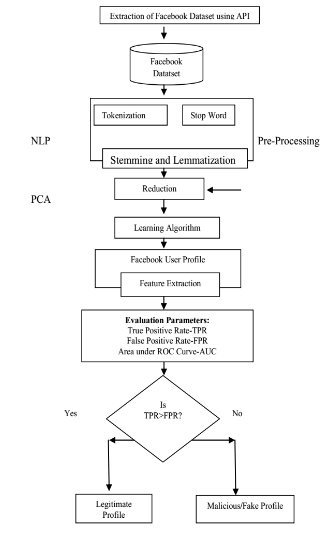
\includegraphics[width=130mm]{DeroulementAlgo.PNG}
    \end{center}
    \caption{Déroulement de l'algorithme}
\label{fig:Déroulement de l'algorithme}
  \end{figure}

\newpage
On constate que l'algorithme se déroule en trois étapes principales : \\
- Le pré-traitement (NLP) \\
- Analyse en composantes principales (PCA) \\
- L'algorithme d'apprentissage \\

Le pré-traitement est essentiel pour réduire au minimum la taille de l'ensemble de données récupérées en préambule et pour renforcer l'efficience (capacité de rendement) et l'efficacité de la méthode. Ce pré-traitement repose sur la "Tokenization" et le "Stop Word".\\

La tokenisation est, d'après Wikipédia, \textit {"le processus consistant à diviser un contenu textuel en phrases, expressions, symboles ou différents facteurs significatifs appelés jetons. Le but de la tokenisation est d'explorer les phrases d'une phrase. La liste des jetons se transforme en entrée pour un traitement ultérieur s'apparentant à l'analyse syntaxique ou à l'exploration de contenu textuel."} La tokenisation est précieuse à la fois en linguistique (où il s’agit d’une forme de segmentation du contenu textuel) et en informatique portative, où elle fait partie de l’analyse lexicale. La connaissance textuelle est plus simple sur un simple bloc de caractères au début. Toutes les stratégies de récupération du savoir-faire nécessitent les mots de l'ensemble de données. Pour cette raison, l'exigence d'un analyseur syntaxique est une tokenisation des enregistrements. Cela peut paraître banal car le texte est déjà enregistré dans des codecs lisibles par un appareil. Cependant, certains problèmes subsistent, tels que la suppression des signes de ponctuation. Différents caractères tels que les crochets, les traits d'union, etc. doivent également être traités.\\
Les phrases d’arrêt (ie Stop Word) sont très souvent utilisées, mais pas forcément utilisées pour la classification des enregistrements. Des mots tels que «et», «sont», «ceci», etc. doivent être enlevés. Cependant, le développement de telles phrases de fin d'enregistrement est problématique et incohérent entre les sources textuelles. Ce processus réduit également la connaissance du texte et améliore les performances de l'approche. Chaque rapport de contenu textuel offre avec ces phrases qui ne sont pas essentielles pour les applications de text mining.\\

Vient ensuite l'étape de la racinisation et de la lemmatisation (Stemming and Lemmatization). \\
La racinisation ou désuffixation est un procédé de transformation des flexions (ensemble des modifications subies par le signifiant des mots, dans ce cas précis au moment de la tokenisation et des phrases d'arrêt) en leur radical ou racine. \\
La lemmatisation désigne un traitement lexical apporté à un texte en vue de son analyse. Ce traitement consiste à appliquer aux occurrences des lexèmes sujets à flexion (en français, verbes, substantifs, adjectifs) un codage renvoyant à leur entrée lexicale commune ("forme canonique" enregistrée dans les dictionnaires de la langue, le plus couramment), que l'on désigne sous le terme de lemme. \\

Vient ensuite le PCA ou l'analyse en composantes principales. L'objectif principal de l'analyse en composantes principales d'après l'article est \textit {"d'extraire les connaissances fondamentales du tableau, de les symboliser comme une suite de nouvelles variables orthogonales connues sous le nom de composants principaux et de montrer l'échantillon de similarité des observations et des variables en tant qu'éléments dans des cartes."} En résumé, le but ici est de réduire au maximum l'ensemble de données que le pré-traitement nous a retourné afin d'avoir uniquement l'essentiel, soit les composantes principales pour la suite.\\

Enfin, on injecte dans le profil de l'utilisateur Facebook que l'on souhaite tester l'ensemble de données retourné par l'analyse en composantes principales et les deux algorithmes cités plus haut qui vont extraire deux paramètres d'évaluation : le taux de vrais positifs et le taux de faux positifs. Si le taux de vrais positifs est supérieur au taux de faux positifs, alors le profil est déclaré légitime, dans le cas contraire, il sera déclaré faux ou malveillant.\\

Ainsi, cet algorithme, que je juge complexe et que j'ai personnellement eu du mal à comprendre au début se base sur des éléments de langage pour s'accomplir. Pour résumer sa démarche, il transforme et classifie des ensembles de données du langage qu'il a extrait de Facebook au moyen de procédés divers comme la tokenisation, les phrases d'arrêt, la lemmatisation, la racinisation et enfin l'analyse en composantes principales afin de n'utiliser que l'essentiel des ensembles de données pour l'étude finale avec les deux algorithmes afin d'augmenter le taux de précision de détection des faux profils qui permettent de mettre en évidence les vrais positifs et les faux positifs concernant le profil étudié. Ce genre d'algorithmes se révèle redoutable dans les cas des harponneurs africains qui maîtrisent mal la langue française.\\

Il existe d'autres algorithmes, un article traitant une étude de détection de faux profils est présent en bibliographie à la fin de ce mémoire, mais ces trois exemples résument bien, selon moi, l'existant informatique actuel.

\section{Critique de l'existant}
Ici, seulement l'existant informatique actuel va être jugé. Trois algorithmes différents ont été expliqués précédemment. Le premier se basait sur l'âge et le sexe, le second sur le lien entre les individus et le dernier utilisait les éléments de langage. On a donc trois grandes dimensions différentes qui sont étudiées. L'existant actuel est donc déjà assez varié, bien que les méthodes restent rares et non fiables à 100\%. \\

Selon moi, cet existant est pertinent, dans le sens où les variables étudiées sont importantes et nécessaires pour établir la véracité ou non d'un profil. Cependant, le point qui me pose en revanche problème, c'est qu'aucune solution proposée n'utilise plusieurs dimensions en même temps et c'est pourquoi, selon moi, les algorithmes manquent de fiabilité encore de nos jours. Il n'est pas déraisonnable de penser qu'énormément d'utilisateurs de nos jours mentent sur leur nom de famille, sur leur âge, et ont des liens avec des personnes insoupçonnables. Pourtant, il n'est pas sensé d'établir un profil comme étant fake si une personne a renseigné un âge incorrect alors que ses autres informations sont correctes. Le troisième algorithme présenté quant à lui, risque de trouver ses limites dans le cas où l'arnaqueur est bel et bien français. \\

Désormais, il me reste à vous présenter mon apport personnel dans la détection des faux profils, et c'est justement les enjeux de la dernière partie.

\chapter{Apport personnel}
\section{Préambule}
L'objectif de cette dernière partie est d'exposer une contribution afin d'enrichir l'existant informatique dans le cadre de la problématique de ce mémoire. On a vu précédemment avec l'analyse de l'existant, qu'aucun algorithme n'utilise plusieurs dimensions en même temps. Ainsi, dans un premier temps, j'avais pensé à proposer un algorithme permettant d'utiliser toutes les variables clés d'un profil de manière simultanée, cependant le fait que les algorithmes proposés soient implémentés d'une manière différente rend cette solution peu envisageable. \\

L'autre solution que j'ai envisagé et qui va finalement être celle retenue est d'utiliser les graphes.

\section{La méthode des graphes}
Ici, il s'agit de passer par les graphes. La théorie des graphes appartient au domaine de la recherche opérationnelle. \\

Dans le domaine mathématique et informatique, un graphe est la donnée d'un ensemble des sommets et d'un ensemble d'arêtes qui relient deux à deux certains des sommets. Un graphe possède deux caractéristiques principales : \\
- son orientation ou non, selon le fait que les arêtes soient munies ou non d'un sens de parcours.\\
- sa pondération ou non, selon le fait que les arêtes soient affectées d'une valeur ou non.

\subsection{Les graphes de référence pour l'apport}
\subsubsection{Les graphes de relations}
Dans cette partie, cinq individus vont être pris pour exemple, Bob, Alice, Romain, Julie et Léo. Les graphes qui vont suivre vont être représentatifs des relations entre ces personnes. 
\subsubsection{Exemple de graphe de relation non-orienté} 
Ici, les relations d'amitié entre les cinq individus nommés plus haut vont être représentées sous forme de graphe non-orienté. \\

\begin{tikzpicture}
    \node (n6) at (1,10) {Bob};
    \node (n4) at (4,8)  {Alice};
    \node (n5) at (8,9)  {Romain};
    \node (n1) at (11,8) {Julie};
    \node (n2) at (9,6)  {Léo};

  \foreach \from/\to in {n6/n4,n4/n5,n5/n1,n1/n2,n2/n4}
    \draw (\from) -- (\to);
\end{tikzpicture}\\

Ce type de graphe correspond au genre de graphes que l'on peut trouver sur Facebook. En effet, pour être ami avec une autre personne, les deux tiers doivent nécessairement s'ajouter mutuellement, le graphe représentatif de cela n'aura donc pas d'orientation.\\
Ici, on peut retenir que Bob est ami avec Alice, qu'Alice est amie avec Romain, Bob et Léo, que Romain est ami avec Alice et Julie, que Julie est amie avec Léo et Romain et enfin, que Léo est ami avec Alice et Julie. On peut également noter, par exemple, que Romain et Bob ont un ami en commum, Alice et que Romain et Léo en ont deux, Alice et Julie. 

\subsubsection{Exemple de graphe de relation orienté simple}
Ici, les relations d'amitié entre les cinq individus nommés plus haut vont être représentées sous forme de graphe orienté simple. \\
\begin{center}
\begin{tikzpicture}[-latex ,auto ,node distance = 2cm and 3cm ,on grid ,semithick ,state/.style ={ circle ,top color =white , bottom color = processblue!20 , draw, processblue , text=blue , minimum width =1 cm}]
\node[state] (A) { Bob };
\node[state] (B) [above left = of A] { Alice };
\node[state] (C) [above right = of A] { Romain };
\node[state] (D) [below right = of A] { Julie };
\node[state] (E) [below left = of A] { Léo };
\path (A) edge [bend left] node[above] {} (B);
\path (B) edge [bend left] node[above] {} (C);
\path (C) edge [bend left] node[above] {} (D);
\path (E) edge [bend left] node[above] {} (C);
\path (E) edge [bend left] node[above] {} (D);
\path (B) edge [bend left] node[above] {} (E);
\end{tikzpicture}
\end{center}

Ce type de graphe correspond au genre de graphes que l'on peut trouver sur Twitter ou Instagram, avec le système de followings et de followers. Contrairement à Facebook, il n'est pas nécessaire d'avoir un ajout double de la part des deux parties pour pouvoir suivre le profil de l'autre. L'orientation du graphe se justifie alors.\\
Ici, on peut apprendre de ce graphe par exemple qu'Alice suit Romain, que Romain suit Julie, que Léo suit Julie, que Bob suit Alice..., ainsi on peut conclure par exemple que Léo et Romain suivent la même personne, à savoir Julie. Ce graphe ne permet pas de mettre en évidence, ou du moins d'établir une hypothèse sur le fait que les personnes se connaissent ou non, puisque l'orientation est simple. 

\subsubsection{Exemple de graphe de relation orienté double}
Ici, les relations d'amitié entre les cinq individus nommés plus haut vont être représentées sous forme de graphe orienté double.\\
\begin{center}
\begin{tikzpicture}[-latex ,auto ,node distance = 3cm and 4cm ,on grid ,semithick ,state/.style ={ circle ,top color =white , bottom color = processblue!20 , draw, processblue , text=blue , minimum width =1 cm}]
\node[state] (A) { Bob };
\node[state] (B) [above left = of A] { Alice };
\node[state] (C) [above right = of A] { Romain };
\node[state] (D) [below right = of A] { Julie };
\node[state] (E) [below left = of A] { Léo };
\path (A) edge [bend left] node[above] {} (B);
\path (B) edge [bend left] node[above] {} (C);
\path (C) edge [bend left] node[above] {} (B);
\path (C) edge [bend left] node[above] {} (D);
\path (D) edge [bend left] node[above] {} (C);
\path (E) edge [bend left] node[above] {} (C);
\path (E) edge [bend left] node[above] {} (D);
\path (B) edge [bend left] node[above] {} (E);
\path (E) edge [bend left] node[above] {} (B);
\end{tikzpicture}
\end{center}

Ce type de graphe correspond toujours au genre de graphes que l'on peut trouver sur Twitter ou Instagram, avec le système de followings et de followers. Cependant, ici, le fait que l'orientation soit double permet de nous apprendre si la personne qui suit une autre personne a été suivie en retour ou non. On apprend, qu'ici, Alice/Romain, Romain/Julie, et Alice/Léo se suivent mutuellement, on peut ainsi établir une éventuelle hypothèse sur le fait que ces derniers se connaissent. 

\subsubsection{Le graphe d'actions}
Contrairement aux graphes précédents qui étaient autour des relations entre profils, ce graphe-ci va présenter, de manière simplifiée, les actions qu'un profil va réaliser sur un réseau social. On va utiliser pour cela un graphe orienté pondéré.
\begin{center}
\begin{tikzpicture}[-latex ,auto ,node distance = 3cm and 4cm ,on grid ,semithick ,state/.style ={ circle ,top color =white , bottom color = processblue!20 , draw, processblue , text=blue , minimum width =1 cm}]
\node[state] (A) { Bob };
\node[state] (B) [above left = of A] { Sport };
\node[state] (C) [above right = of A] { Cuisine };
\node[state] (D) [below left = of A] { Politique };
\node[state] (E) [below right = of A] { Vêtements F };
\path (A) edge [bend left] node[above] {$76$} (B);
\path (A) edge [bend left] node[above] {$25$} (C);
\path (A) edge [bend left] node[above] {$37$} (D);
\path (A) edge [bend left] node[above] {$2$} (E);
\end{tikzpicture}
\end{center}
Ici, ce sont les actions de Bob du mois dernier qui sont tracées via ce graphe. La pondération représente le nombre de fois que ce dernier a consulté ou commenté sur un réseau social des pages ou comptes en rapport avec le domaine inscrit sur le sommet associé. 

\subsection{Explications de l'apport}
Il a été présenté, précédemment, différents graphes qui vont servir de support pour les explications de mon apport. Les graphes représentent, selon moi, un outil pouvant potentiellement être très puissant dans la détection des faux profils, et je vais vous expliquer pourquoi dans cette sous-partie.

\subsubsection{Les graphes de relations}
Les graphes de relations permettent de schématiser de manière simple les relations existant entre différents profils. Afin de se révéler efficace, ce type de graphe va notamment se baser sur le concept d'amis en communs que l'on trouve sur Facebook.\\
En effet, avec le premier graphe de relation, on a pu établir que Romain et Bob ont un ami en commum, Alice et que Romain et Léo en ont deux, Alice et Julie. Ainsi, on peut conclure que Romain et Bob sont liés par Alice et Romain et Léo sont liés par Alice et Julie. Plus des profils auront des amis en communs, plus ces derniers seront liés et plus ces derniers seront moins suspects. Il a également été dit, lorsque les moyens de détection naïfs des profils ont été explicités, qu'un escroc prendra rarement la peine d'établir un véritable réseau solide, principalement par faute de temps. Ainsi, si un profil en particulier se dégage par le fait qu'il n'est pas d'ami en commun et qu'il soit isolé des autres profils, cela peut paraître suspect. Dans notre exemple, Bob serait potentiellement suspect, car il est ami avec Alice mais est totalement isolé du reste du réseau. \\
Il a également été dit qu'il est monnaie courante qu'un escroc établisse un faux réseau de quelques personnes, toutes fakes, afin d'augmenter sa crédibilité auprès de ses victimes. Les graphes d'actions se révéleraient très utiles dans ce genre de cas car ils permettraient de repérer de manière simple un groupe de profils s'étant ajouté mutuellement mais n'ayant aucun autre ami à côté. \\

Les deux autres graphes de relations, ceux orientés, permettent de mettre la lumière sur les faux profils de manière similaire mais également de manière différente. En effet, comme évoqué précédemment, avec ces graphes, l'ajout réciproque n'est pas obligatoire, c'est le cas de figure que l'on peut par exemple trouver sur Twitter ou Instagram avec le système d'abonnements et d'abonnés. Repérer un faux profil avec la même manière que pour un cas où l'ajout réciproque est obligatoire peut toujours se faire, mais cela sera forcément plus compliqué. En revanche, la non-réciprocité obligatoire de l'ajout permet d'utiliser une autre méthode, celle des clusters informatiques. Pour la définition, il s'agit de groupes de serveurs indépendants fonctionnant comme un seul et même système. Le but ici est de jouer sur le fait que deux profils ayant le même sexe, un âge similaire, venant d'une classe sociale similaire, ayant une origine commune etc... fonctionnent d'une manière plus ou moins identique, suivent les mêmes profils et forment ainsi, un seul et même réseau bien qu'ils soient indépendants au départ. Par exemple, il est logique que deux adolescentes suivent Ariana Grande, une superstar actuelle de la pop sur Instagram ou Twitter. Ainsi, le but ici serait de débusquer un profil ne rentrant pas dans un réseau "habituel" et de le déclarer comme étant suspect. 

\subsubsection{Le graphe d'actions}
Le graphe d'action permet de suivre de manière très efficace  l'activité d'un profil. Avec l'exemple donné, on constate que Bob, le mois dernier, a consulté ou commenté environ deux fois plus de comptes ou de pages à vocation sportive qu'à vocation politique. On remarque également qu'il a seulement consulté que deux fois des comptes ou pages en rapport avec des vêtements féminins. \\

On comprend ainsi assez aisément tout l'enjeu de cette méthode dans la détection de faux profils. En effet, en récoltant et en traçant l'activité d'un profil, on peut comparer la réalité avec la théorie. On peut également établir des hypothèses sur les actions d'un profil en fonction des informations saisies sur ce dernier mais aussi de repérer les profils suspects. \\

En effet ici, il semble tout à fait logique que Bob ait consulté ou commenté le mois dernier seulement 2 fois des pages ou comptes en rapport avec les vêtements féminins, étant donné qu'il s'agit d'un homme. Si le nombre de consultations ou de commentaires aurait été élevé, on aurait pu établir le profil de Bob comme étant suspect. Un autre exemple que l'on pourrait citer est par exemple, d'observer une personne qui se dit avoir 20 ans être active sur des groupes où l'on discute de la retraite. Les graphes d'actions se révéleraient donc utiles pour repérer des profils suspects mais également, même si cela sort du cadre de ce mémoire, pour établir des estimations sur les activités des personnes en fonction de leur âge, de leur sexe, ou encore de leur classe sociale. Ici, la méthode des clusters évoquée pour les graphes de relations serait toujours valable : deux personnes ayant saisies des informations similaires sur leur profil respectif aurait tendance à avoir une activité plus ou moins similaire. Le cas échéant, si l'on trouve un profil ne respectant pas cela, ce dernier pourrait être éventuellement déclaré comme étant suspect.

\section{Critique de l'apport}
La méthode des graphes est intéressante car elle permet de mettre en avant les enjeux de véracité d'un profil de manière simple et compréhensible pour un individu lambda. Cette méthode peut selon moi être extrêmement puissante car elle permet de facilement isoler un profil ou un groupe de profils suspect via les graphes de réseau et de facilement détecter les profils ayant des activités ne correspondant pas aux informations qu'ils ont saisies via les graphes d'actions. \\

Cependant, cette méthode peut trouver selon moi ses limites dans le fait que certaines personnes ne rentrent volontairement pas des informations de profil véridiques dans le but de ne pas partager des informations qu'elles jugent privées ou qu'elles veulent garder secrètes afin de préserver leur tranquillité comme notamment l'âge ou le sexe et cela peut compromettre l'efficacité de cette méthode, dans le sens où un profil pourrait être déclaré comme étant faux et surtout malveillant alors qu'il ne l'est en réalité pas et ainsi d'augmenter le taux de faux positifs.\\ 
Il faut également prêter attention aux événements particuliers, pour reprendre notre exemple de pages ou comptes de vêtements féminins le mois de la Saint-Valentin ou de la fête des mères, il ne serait guère illogique que l'activité d'un homme sur ce genre de pages connaisse une importance hausse et par conséquent, apporterait une quantité importante de faux positifs.\\
Par ailleurs, le fait qu'il soit tout à fait possible que deux personnes n'ayant aucun point commun peuvent avoir un lien peut également compromettre la fiabilité de la méthode. \\
Se pose aussi la question du passage à l'échelle. Les graphes ont le comportement attendu pour un faible nombre de profils mais cela serait-il toujours le cas pour des centaines de milliers de profils ? \\

Néanmoins, les graphes pour ma part, restent une solution parfaitement viable et trouvent leur principal avantage dans le fait qu'ils soient facilement compréhensibles pour tous, là ou on ne peut pas en dire de même avec des algorithmes.

\chapter{Conclusion}
Ce mémoire a trouvé sa raison d'être autour des réseaux sociaux qui sont une sous-catégorie des médias sociaux. Ces outils puissants apportent énormément d'intérêt, le principal étant la communication. En effet, le réseau social a radicalement changé notre manière de communiquer. Cependant, un individu peut facilement perdre le contrôle de son identité numérique. Il est même raisonnable de penser que l'on en a jamais véritablement le contrôle, puisque ce que l'on fait sur les réseaux sociaux reste en mémoire, et ce, même si l'on supprime nos traces. L'exemple de Facebook parait le plus parlant, car un compte, même désactivé, reste dans la base de données du géant américain et n'est par conséquent jamais totalement supprimé pour eux, ce qui rend le droit à l'oubli difficile à obtenir. \\

L'identité numérique, citée plus haut, est centrale sur les réseaux sociaux. Elle possède des caractéristiques diverses, parfois complexes, qui permettent d'établir la carte d'identité d'un individu sur Internet. Elle joue la plupart du temps un rôle crucial, par exemple dans le processus du recrutement, les recruteurs vont en effet, utiliser le profil d'un réseau social de la personne comme un élément important du recrutement éventuelle de cette dernière. Il faut ainsi faire bien attention à ce que l'on dit, fait, achète, publie, montre sur les réseaux sociaux. Certaines personnes ont conscience de cela et utilise ainsi leur identité numérique afin de se glorifier et "d'arranger la réalité" notamment dans le cadre d'un recrutement.\\

Avoir une identité numérique comporte des risques, l'usurpation d'identité étant l'un des principaux. A cause d'Internet, usurper une identité est devenu encore plus facile qu'auparavant. L'usurpation d'identité numérique se distingue de celle classique, car là où on se faisait passer pour quelqu'un dans le but de lui escroquer de l'argent dans l'usurpation classique, celle numérique peut aussi avoir un but de sabotage de réputation. L'usurpation d'identité numérique peut également trouver sa raison d'être dans le fait de vouloir tromper les autres : se faire passer pour quelqu'un d'autre afin de gagner la confiance d'une personne, en ayant recours très souvent au domaine sentimental et de lui soutirer des photos et vidéos intimes afin de lui réclamer de l'argent ensuite sous peine de divulguer aux proches de la victime ces dites photos et vidéos. Cette recherche de vouloir duper autrui peut aussi se faire en se créant un faux profil afin de profiter de la crédulité de la victime qui pensera parler à quelqu'un d'autre alors qu'elle parle en réalité à une personne qui "n'existe pas".\\

Cette dimension de faux profil se distingue de la dimension de faux compte par deux manières : la première étant que le faux profil sera géré par une personne humaine alors que le faux compte sera certes programmé par une personne humaine mais géré par un robot ou bot. La seconde est qu'un faux compte trouvera sa raison d'être dans le fait de vouloir influencer les personnes qui ont accès à son contenu, comme par exemple pour les bots Twitter, via des retweets d'expressions similaires, ou encore dans le fait de proposer des services, comme les bots Discord, ou certains comptes Twitter, qui corrige les utilisateurs du réseau social faisant des fautes dans leurs tweets sur l'orthographe français des Pokemon. Le faux profil, lui, sera soit dans un but de conservation d'anonymat, soit dans un but matrimonial, soit dans un but de tromperie d'un tiers. Cette notion de tromperie fait naître la dimension malveillante du faux profil, notion que l'on ne trouvera pas dans le faux compte, malgré le caractère malhonnête de certains utilisant des processus de manipulation comme l'astroturfing.\\

Les réseaux sociaux luttent pour pouvoir tenter d'endiguer l'hémorragie du faux profil, principalement dû à son caractère très souvent malveillant. Des solutions existent, les plus connues sont non informatiques, elles peuvent être utilisées par tout utilisateur lambda, quant à celles informatiques, elles reposent sur des dimensions précises comme l'âge, le sexe, le lien existant entre les individus ou les éléments du langage. L'apport proposé consiste de passer par les graphes, afin d'isoler des profils ou groupes de profils n'ayant aucun réseau ou encore de repérer des profils n'ayant pas une activité attendue au regard des informations qui ont été saisies sur ce dernier.\\

Les solutions existantes trouvent leurs limites et ne sont évidemment pas fiables à 100\%. Néanmoins, elles restent tout de même dans énormément de cas, des solutions viables, surtout si la personne à l'origine du faux profil n'est pas une professionnelle.\\
Quant à ma solution personnelle, elle n'a pas pu être testée donc il est impossible, au moment de la rédaction de ce mémoire, d'émettre un réel jugement sur la viabilité de cette méthode. \\

Le plus important reste d'être prudent et toujours méfiant dans la jungle aux profils que l'on trouve sur les réseaux sociaux. Le but des faux profils et de certains faux comptes est justement de gagner la confiance de leurs victimes, avoir des doutes sur les intentions des personnes qui surgissent de nulle part est selon moi l'attitude minimaliste à adopter. Ce proverbe d'Aristote me semble idéal pour conclure \textit {"Le doute est le commencement de la sagesse."}

\nocite{*}
\printbibliography

\end{document}
